In this section, we formally state our synthesis problem. 

\newcommand{\Op}{\mathit{Op}}
\newcommand{\of}{\mathbf{of}}
\newcommand{\matchc}{\mathbf{match}}
\newcommand{\withc}{\mathbf{with}}
\newcommand{\zug}[1]{\langle  #1 \rangle}
\newcommand{\rec}{\mathbf{rec}}


\begin{figure*}[t]
\vspace{-0.15in}
\begin{center}
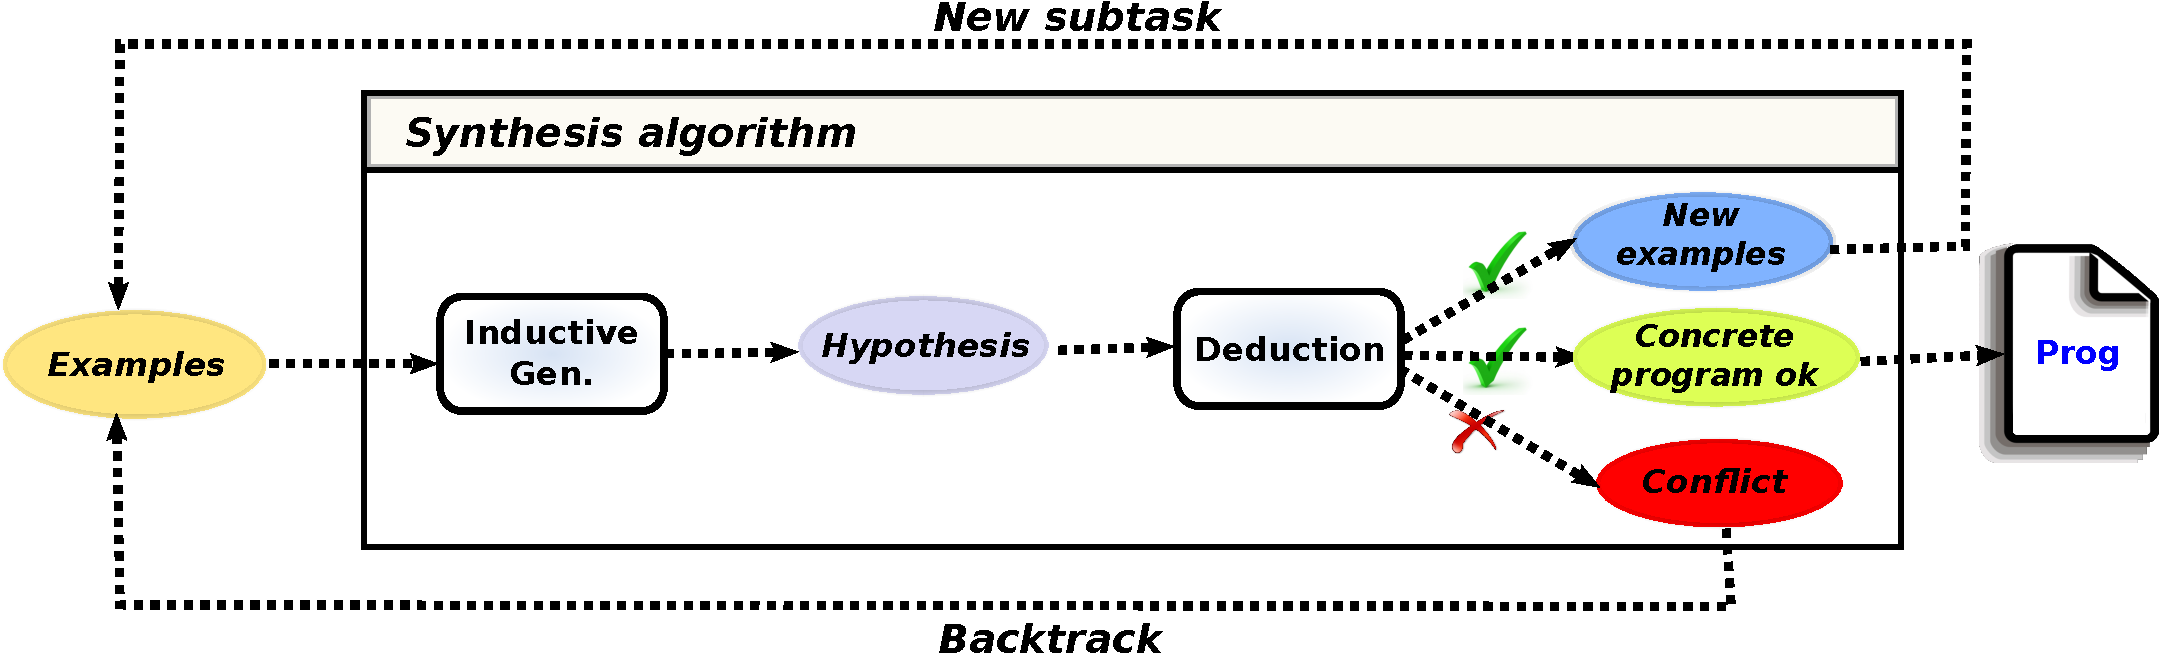
\includegraphics[scale=0.37]{overview-modified3.pdf}
\end{center}
\caption{High-level overview of our synthesis
  algorithm}\label{fig:overview}
\vspace{-0.1in}
\end{figure*}

\paragraph{Programming language} 

Our method synthesizes programs in a $\lambda$-calculus with algebraic
types and recursion. Let us consider {\em signatures} $\zug{\Op,
  \id{Const}, \cal{A}}$, where $\Op$ is a set of {\em primitive
  operators}, $\id{Const}$ is a set of constants, and $\cal{A}$ is a
set of equations that relate operators and constants.  The syntax of
programs $e$ over such a signature is given by:
\begin{eqnarray*} e & ::= & x \mid c \mid \lambda x. e' \mid e_1~e_2 \mid \rec~f.(\lambda x. e')
 \mid (e_1,e_2) \mid \oplus~e' \mid \\
 & & \{ l_1: e_1,\dots, l_k: e_k \} \mid e'.l \mid \zug{l_i(e_i)} \mid \\
  & & \matchc~e'~\withc~\zug{l_1(x_1) \Rightarrow
    e_1',\dots, l_k(x_k) \Rightarrow
    e_k'} 
\end{eqnarray*}

Here, $x$ and $f$ are variables, $\oplus \in \Op$, and $c \in \id{Const}$.
% is a {\em primitive
%  operator} and $c$ is a {\em constant}. Operators and constants are
%assumed to be related by an equational theory that rules, for
%instance, that $2 + 2 = 4$. 
The syntax has standard meaning; in particular:
\begin{enumerate}
\item $\rec~f.(\lambda x. e)$ is a recursive function $f$.

\item $e = \{ l_1: e_1,\dots, l_k: e_k \}$ is a record whose
field $l_i$ has value $e_i$. We have $e.l_i = e_i$.

\item $e = \zug{l_i(e_i)}$ is a variant labeled $l_i$. The construct
  ``$\matchc~e~\withc~\dots$'' performs ML-style pattern-matching. 
\end{enumerate}
We assume the standard definition of free variables. A
program is {\em closed} if it does not have any free variables.

As the operational semantics of the language is standard, we do not
discuss it in detail. We simply assume that we have a relation $\leadsto$
such that $e_1 \leadsto e_2$ whenever $e_1$ evaluates to $e_2$ in one
or more steps. 
%A program is {\em irreducible} if it does not evaluate
%to a program other than itself.
Our programs are typed using an ML-style polymorphic type system. Since this
system is standard,  we skip a detailed description.

Our implementation of the language comes prepackaged with certain
primitive operators, constants, and type definitions. Predefined types
include (polymorphic) lists and trees, encoded as variants.
Predefined operators include the standard arithmetic operators,
if-then-else, and higher-order combinators like {\tt map}, {\tt
  foldl}, {\tt foldr}, and {\tt foldt} (see Figure~\ref{fig:abstract-hypotheses}). In a particular synthesis
task, we may augment this set with {\em external} operators, constants
and types. For instance, in the synthesis of the \verb+selectnodes+
function in \secref{selectnodes}, {\tt pr} is an external operator.


\newcommand{\C}{\mathcal{C}}
\paragraph{Cost model}

Each program $e$ in the language has a {\em cost} $\C(e) \ge 0$.  This
cost is defined inductively. Specifically, we assume that each
primitive operator $\oplus$ and constant $c$ has a known, positive
cost. Costs for more complex expressions satisfy constraints like the
following (we skip some of the cases for brevity):
\begin{itemize}
\item $\C(\oplus~e) > \C(\oplus) + \C(e)$
\item $\C(\lambda x. e) > \C(e)$ 
\item $\C(e_1~e_2) > \C(e_1) + \C(e_2)$
\item $\C(x) = 0$. Intuitively, we assign costs to the {\em definition},
  rather than the {\em use}, of variables.
\end{itemize}



\paragraph{The synthesis problem}

Let an {\em input-output example} be a term $a_i \mapsto b_i$, where
$a_i$ and $b_i$ are closed programs. The input to our synthesis
problem is a set $\E_{in}$ of such examples. Our goal is to
compute a {\em minimal-cost} closed program $e$ 
%(often called the {\em target program}) 
that {\em satisfies} the examples --- i.e., for each $i$, we have $(e~a_i)
\leadsto b_i$. In what follows, we refer to $e$ as the \emph{target program}.

Note that this problem formulation biases our synthesis procedure towards
generating simpler programs. For example, since our implementation associates a higher cost 
with the {\tt match} %$\matchc~\dots~\withc~\dots$ 
construct than the \verb+fold+ %and \verb+foldr+
operators, our implementation favors fold-based implementations of list-transforming programs
over those that use pattern-matching.

%As an example, our implementation is
%designed to favor fold-based implementations of functions over lists
%over ones that use explicit pattern-matching. This is done by setting
%the cost for our ``$\matchc~\dots~\withc~\dots$'' construct to be
%adequately higher than the costs of the \verb+foldl+ and \verb+foldr+
%operators.

\paragraph{Hypotheses} The concept of {\em hypotheses} about the
structure of the target programs is key to our approach. Intuitively,
a hypothesis is a program that may have placeholders for missing
expressions. Formally, a {\em hypothesis} is a program that possibly
has free variables. Free variables in a hypothesis are also known as
{\em holes}, and a hypothesis with holes is said to be {\em open}. For
instance, $x$ and $\lambda x. f^* x$ are open hypotheses. In contrast, 
hypotheses that do not contain free variables are said to be \emph{closed}. 
For example, $\lambda x. \ {\tt map} \ (\lambda y. \ y+1) \ x$ is a closed hypothesis.

A hypothesis $h$ is typed under a {\em typing context} that assigns
types to its holes. Given a type $\tau$, we say that $h$ is {\em
  consistent} with $\tau$ if there exists a typing context under which
the type of $h$ equals $\tau$. This property can be decided using a 
standard type inference algorithm.
